\documentclass[12pt,a4paper,oneside,brazil]{abntex2}

% Pacotes que serão utilizados%
\usepackage{lmodern}
\usepackage[utf8]{inputenc}
\usepackage[brazil]{babel}
\usepackage[T1]{fontenc}
\usepackage{indentfirst}
\usepackage{graphicx}
\usepackage{microtype}
\usepackage[backend = biber, style=abnt]{biblatex}
\addbibresource{Referencias.bib}

% Informações do documento %
\title{Notas Introdução a econometria}
\author{Thiago Oliveira Coelho}
\date{\today}



\begin{document}
\pagestyle{plain}
\pagenumbering{arabic}

\maketitle
\begin{center}
Resumo baseado em: \cite{gujarati}, \cite{wooldridge} e \cite{magalhaes}
\end{center}
\tableofcontents

\chapter{1ª Unidade}
\section{Terminologia estatística}
\begin{itemize}
\item População : conjunto total sobre o qual se quer fazer inferências;
\item Amostra: Subconjunto da população que é coletado para fim de realizar análises e fazer estas inferências.
\item Variável aleatória: uma variável que pode assumir diferentes valores dependendo do resultado do experimento. Pode ser:
\begin{itemize}
\item Discreta: assume valores finitos; (EX: 1; 2; 3; 4...)
\item Contínua: assume incontáveis valores. (EX: 1; 1,0001; 1,0002....)
\end{itemize}
\end{itemize}

\section{Somatório}
Considere uma sequência de observações, cada uma representada por um subscrito:
\[ X_i, i = 1,2,3,4,...,n\]
Podemos somar os valores os valores individuais de cada observação X da seguinte maneira:
\[ \sum_{i=1}^{n} X_i\]
Soma os valores de $X$ a partir de $i =1$ até $i =n$.

\subsection{Propriedades do somatório}

\begin{itemize}
\item Sendo $C$ uma constante:
\[\sum_{i=1}^{n} C = n C \]
\item Variável indexada por constante:
\[ \sum_{i=1}^{n} C X_i = C \sum_{i=1}^{n} X_i \]
\item Soma de duas sequências:
\[ \sum_{i=1}^{n} (X_i + Y_i) = \sum_{i=1}^{n} X_i + \sum_{i=1}^{n} Y_i \]
\item O somatório de uma razão não é a razão dos somatórios:
\[ \sum_{i=1}^{n} \frac{X_i}{Y_i} \neq \frac{\sum_{i=1}^{n} X_i}{\sum_{i=1}^{n} Y_i} \]
\item Soma dos quadrados não é igual ao quadrado das somas:
\[ \sum_{i=1}^{n} X_i^2 \neq (\sum_{i=1}^{n} X_i)^2 \]
 \end{itemize}
 
 \section{Desvios com relação a média}
 \begin{itemize}
 \item Média amostral:
\[ \overline{X} = \frac{\sum_{i=1}^{n} X_i}{n}\]
\item Mediana: valor correspondente da observação que divide a quantidade da amostra em duas partes iguais;
\item Variância: mostra quão longe da média estão os valores das observações:
\[ \sigma^2 = \frac{\sum_{i=1}^{n} (X_i - \overline{X})^2}{n-1} \]
\item Desvio padrão: indica quão uniforme é um conjunto de dados:
\[ \sigma = \sqrt{\sigma^2} \]
 \end{itemize}
 
\section{Logaritmo natural}
É um logaritmo que tem como base o número de euler $e = \approx 2,71828$.

\begin{figure}[h]
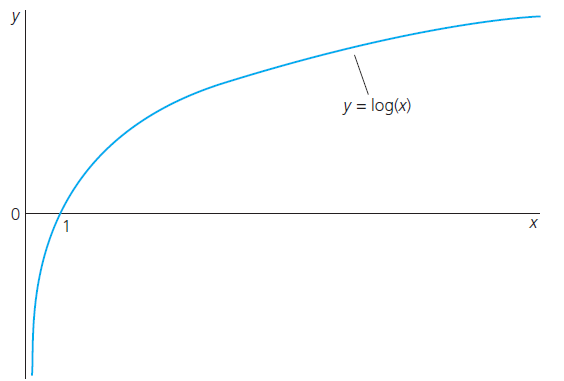
\includegraphics[scale=0.7]{logaritmo natural.png}
\centering
\caption{Fonte: \cite[p. 637]{wooldridge}}
\end{figure}

 Possui as seguintes propriedades:
\begin{itemize}
\item $ln (X_1 X_2) = ln X_1 + ln X_2 $;
\item  $ln \frac{X_1}{X_2} = ln X_1 - ln X_2$;
\item  $ln X_1^{\alpha } = \alpha ln X_1$;
\item $ ln X_2 - X_1 \approx \frac{X_2 - X_1}{X_1} = \frac{\triangle X}{X_1} = \triangle \% X $
\end{itemize}

\section{Função exponencial natural}
É aquela função exponencial cuja base é o número de euler. É o inverso da função logaritmo natural, perceba pelo gráfico:

\begin{figure}[h]
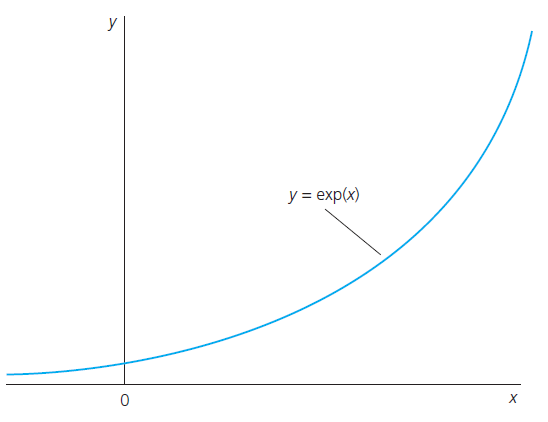
\includegraphics[scale=0.7]{exponencial natural.png}
\centering
\caption{Fonte: \cite[p. 640]{wooldridge}}
\end{figure}

\chapter{2ª Unidade}
\section{Probabilidade}
\printbibliography
\end{document}
